\bookchapter{Capítulo 42: Panorama dos grandes modelos e prática de API}

\chapterintro{Os capítulos anteriores foram sobre “como colaborar com a IA”; este resolve uma pergunta mais básica: “qual IA usar e como?”. Em agosto de 2026, o mercado é riquíssimo: no exterior, GPT, Claude e Gemini disputam o topo; na China, DeepSeek, Qwen, GLM, Kimi e Doublo florescem. Cada modelo tem personalidade e especialidade: a escolha certa multiplica resultados; a errada, atrapalha. Aqui você vai conhecer esses modelos, conectá-los às suas aplicações por API e escolher o plano de tokens certo.}

\booksection{Principais modelos internacionais: o trio de liderança}

Em agosto de 2026, o mercado internacional se consolidou em torno de OpenAI (GPT), Anthropic (Claude) e Google (Gemini). Cada um com um perfil marcado — vamos um a um.

\booksubsection{OpenAI GPT-5.6: o atleta completo}

A OpenAI abriu a onda dos grandes modelos e a série GPT continua sendo a mais usada no mundo. Lançada em julho de 2026, a família GPT-5.6 tem três perfis: GPT-5.6 Sol (topo de linha para raciocínio avançado), GPT-5.6 Terra (equilibrado para o dia a dia) e GPT-5.6 Luna (leve e de baixo custo para alta concorrência). Os três compartilham janela de contexto de 1,05 milhão de tokens e suportam entrada de imagem, chamadas de função e saída estruturada.

\begin{center}
\begin{tabularx}{\linewidth}{|X|X|X|X|X|}
\hline
\textbf{Modelo} & \textbf{Posicionamento} & \textbf{Entrada (por milhão de tokens)} & \textbf{Saída (por milhão de tokens)} & \textbf{Janela de contexto} \tabularnewline
\hline
GPT-5.6 Sol & Raciocínio de topo & US\$ 5,00 (cerca de 36 yuan) & US\$ 30,00 (cerca de 217 yuan) & 1,05 milhão de tokens \tabularnewline
GPT-5.6 Terra & Equilibrado para o dia a dia & US\$ 2,50 (cerca de 18 yuan) & US\$ 15,00 (cerca de 109 yuan) & 1,05 milhão de tokens \tabularnewline
GPT-5.6 Luna & Leve e econômico & US\$ 1,00 (cerca de 7 yuan) & US\$ 6,00 (cerca de 44 yuan) & 1,05 milhão de tokens \tabularnewline
\hline
\end{tabularx}
\end{center}

\begin{center}\small\color{gray}Preços da série OpenAI GPT-5.6 (agosto de 2026)\end{center}

A grande força do GPT é o equilíbrio: raciocínio, programação, escrita e multimodal sem fraqueza evidente. Somados o vasto ecossistema de plugins e a comunidade, a documentação e a cadeia de ferramentas são as mais completas. Para quem “não sabe o que escolher”, o GPT é a resposta segura. Limites: na China exige rede especial, o chinês por vezes soa “traduzido” e a API fica na faixa média-alta.

\textbf{Boa notícia}\par

Em agosto de 2026, a OpenAI anunciou que o modelo padrão para usuários gratuitos passou a ser o GPT-5.6 Luna, com chat de texto ilimitado. Ou seja, dá para experimentar as capacidades básicas sem custo e pagar só quando precisar de raciocínio mais forte ou de API.

\booksubsection{Anthropic Claude: o topo em programação e rigor}

Se o GPT é o atleta completo, o Claude é o “teto” da programação. A série Claude da Anthropic lidera com folga no SWE-bench (benchmark de engenharia de software) e tem a melhor qualidade de código e capacidade de entrega em projetos reais. Raro ainda: a taxa de alucinação é a mais baixa do mercado, cerca de 1\% — ideal para cenários de alta precisão, como academia e jurídico.

Outra carta forte é o contexto longo: janela de 1 milhão de tokens, capaz de “ler” contratos de centenas de páginas ou um repositório inteiro sem perder detalhes. Quase insubstituível em refatoração e análise de documentos longos. O Claude Code, ferramenta de terminal, chegou a US\$ 2,5 bilhões anuais em meados de 2026 — a maior prova do reconhecimento da capacidade de programação do Claude.

\begin{center}
\begin{tabularx}{\linewidth}{|X|X|X|X|X|}
\hline
\textbf{Modelo} & \textbf{Posicionamento} & \textbf{Entrada (por milhão de tokens)} & \textbf{Saída (por milhão de tokens)} & \textbf{Janela de contexto} \tabularnewline
\hline
Claude Fable 5 & Topo de linha & US\$ 10,00 (cerca de 72 yuan) & US\$ 50,00 (cerca de 362 yuan) & 1 milhão de tokens \tabularnewline
Claude Opus 4.8 & Profissional & US\$ 5,00 (cerca de 36 yuan) & US\$ 25,00 (cerca de 181 yuan) & 1 milhão de tokens \tabularnewline
Claude Sonnet 5 & Custo-benefício & US\$ 2,00 (cerca de 14 yuan) & US\$ 10,00 (cerca de 72 yuan) & 1 milhão de tokens \tabularnewline
\hline
\end{tabularx}
\end{center}

\begin{center}\small\color{gray}Preços da série Anthropic Claude (agosto de 2026; Sonnet 5 em preço promocional)\end{center}

O ponto fraco é o preço: a saída do Fable 5 é a mais cara de todas, US\$ 50 por milhão de tokens. A parte multimodal (imagem e vídeo) também é mais fraca. Para desenvolvedores individuais com orçamento apertado, o Sonnet 5 em promoção tem excelente custo-benefício.

\booksubsection{Google Gemini: o rei do multimodal}

A série Gemini do Google chegou em 2026 à versão 3.1 Pro. Seu trunfo é o multimodal nativo: análise precisa de imagem e texto, OCR de tabelas sem erro, extração eficiente de quadros de vídeo e análise profunda de áudio e vídeo. Integrada ao ecossistema Google (busca, e-mail, nuvem), destaca-se em informação em tempo real e compreensão entre modalidades. Suporta ainda 2 milhões de tokens — a maior janela do mercado.

O Gemini é “primeira opção em raciocínio científico e multimodal”. Em projetos com muita imagem, vídeo ou computação científica, quase não tem rival. Em código em texto puro, fica um pouco atrás do Claude; e o chinês não soa tão natural quanto os modelos chineses.

\begin{center}
\begin{tabularx}{\linewidth}{|X|X|X|X|}
\hline
\textbf{Item de comparação} & \textbf{GPT-5.6} & \textbf{Claude Fable 5} & \textbf{Gemini 3.1 Pro} \tabularnewline
\hline
Pontuação geral & 94.8 & 95.0 & 92.1 \tabularnewline
Programação (SWE-bench) & 74.9\% & 64.3\% (Pro) & Médio \tabularnewline
Janela de contexto & 1,05 milhão de tokens & 1 milhão de tokens & 2 milhões de tokens \tabularnewline
Multimodal & Equilibrado & Mais fraco & O mais forte \tabularnewline
Taxa de alucinação & Baixa & A mais baixa (cerca de 1\%) & Baixa \tabularnewline
Disponibilidade na China & Exige rede especial & Exige rede especial & Exige rede especial \tabularnewline
Ecossistema de API & O mais completo & Em crescimento & Vinculado ao ecossistema Google \tabularnewline
\hline
\end{tabularx}
\end{center}

\begin{center}\small\color{gray}Comparação entre os três grandes modelos internacionais (agosto de 2026)\end{center}

\begin{tcbwarn}{Atenção: os obstáculos práticos para usar dentro da China}
Para os desenvolvedores dentro da China, o principal obstáculo a GPT, Claude e Gemini é o acesso à rede. Dá para usá-los indiretamente por meio de proxies Azure, plataformas agregadoras de API e afins, mas a estabilidade e a conformidade precisam ser avaliadas por conta própria. Se o seu projeto tem requisitos rígidos de segurança de dados, a recomendação é priorizar os modelos nacionais.

\end{tcbwarn}

\booksection{Os principais grandes modelos nacionais: diversidade florescente}

Em 2026, os grandes modelos nacionais deixaram de ser 'perseguidores' e viraram 'corredores lado a lado', chegando a 'liderar' em algumas áreas. Diferente da polêmica dos 'wrappers' de 2023, os modelos nacionais de ponta de 2026 já empatam com os melhores modelos internacionais em raciocínio lógico, geração de código e compreensão do chinês, com uma diferença reduzida a menos de 5\%. Mais importante: os modelos nacionais têm vantagens insubstituíveis em cenários com a língua chinesa, em preço e em implantação em conformidade.

\booksubsection{DeepSeek V4: o rei do custo-benefício}

A DeepSeek (Shendu Qiusuo) é um fenômeno entre os grandes modelos nacionais. No começo de 2025, o DeepSeek-V3 chocou o mercado ao se posicionar como 'um décimo do preço do GPT com capacidade equivalente' e ficou conhecido no setor como a 'linha de execução' dos grandes modelos de IA de uso geral — quem custa menos que ele não é tão bom assim, e quem custa mais não entrega o mesmo volume com tanta fartura. Em agosto de 2026, chegou a versão oficial do DeepSeek V4-Pro: arquitetura MoE com 1,6 trilhão de parâmetros, cerca de 49B ativados por chamada e contexto de 1 milhão sem perdas; seu custo-benefício em código é amplamente considerado o teto mundial.

O DeepSeek V4 deu um salto enorme nas capacidades de agente — o benchmark DeepSWE saltou de 12,8 para 62,7 (+390\%) e o NL2Repo subiu de 38,5 para 61,5. A API passou a suportar o protocolo duplo Responses API e Anthropic API, já compatível com ferramentas de programação populares como Codex e Claude Code. Na prática, você pode usar a API do DeepSeek no lugar da API da Claude dentro do Claude Code — o custo cai várias vezes e a experiência é praticamente a mesma.

\begin{center}
\begin{tabularx}{\linewidth}{|X|X|X|X|X|}
\hline
\textbf{Modelo} & \textbf{Posicionamento} & \textbf{Entrada (/1M de tokens)} & \textbf{Saída (/1M de tokens)} & \textbf{Janela de contexto} \tabularnewline
\hline
DeepSeek V4 Pro & Raciocínio de ponta & 3 yuans (cerca de US\$ 0,43) & 6 yuans (cerca de US\$ 0,87) & 1 milhão de tokens \tabularnewline
DeepSeek V4 Flash & Leve e rápido & 1 yuan (cerca de US\$ 0,14) & 2 yuans (cerca de US\$ 0,28) & 1 milhão de tokens \tabularnewline
\hline
\end{tabularx}
\end{center}

\begin{center}\small\color{gray}Preços da série DeepSeek V4 (agosto de 2026, preços promocionais)\end{center}

Comparação de preços: para os mesmos 1 milhão de tokens de entrada + 1 milhão de tokens de saída, o DeepSeek V4 Flash custa cerca de US\$ 0,42, o GPT-5.6 Sol custa cerca de US\$ 35 e o Claude Fable 5 custa cerca de US\$ 60. A diferença chega a 80 a 140 vezes.

\textbf{Cuidado com a cilada: o DeepSeek vai subir de preço}\par

Em 6 de agosto de 2026, a DeepSeek anunciou oficialmente que 'planeja elevar substancialmente os preços da API em breve'; os preços promocionais podem não durar muito. Parte da imprensa especula um aumento de até 30 vezes; até 14 de agosto a empresa ainda não tinha divulgado o plano final de reajuste. Além disso, a versão oficial do DeepSeek V4 introduziu preços por horário de pico — nas horas de pico, o preço das chamadas dobra. Vale acompanhar os anúncios oficiais para saber os preços mais recentes.

\booksubsection{Tongyi Qianwen Qwen3.7 Max: a escolha corporativa do Alibaba Cloud}

A série Tongyi Qianwen (Qwen), do Alibaba Cloud, apoia-se no ecossistema do Alibaba Cloud e tem vantagem natural em implantações corporativas. O Qwen3.7 Max, de julho de 2026, é a atual versão de ponta: modelo denso de 235B de parâmetros, com contexto nativo de 256K, expansível até 1M. As grandes vantagens do Qwen: ecossistema de código aberto maduro (toda a série, do 7B ao 235B, é aberta), compreensão precisa de cenários em chinês e integração profunda com a infraestrutura do Alibaba Cloud.

\begin{center}
\begin{tabularx}{\linewidth}{|X|X|X|}
\hline
\textbf{Modelo} & \textbf{Preço de saída (/1M de tokens)} & \textbf{Cenários de uso} \tabularnewline
\hline
qwen-turbo & 0,6 yuan & Perguntas e respostas simples, classificação de texto e alta concorrência \tabularnewline
qwen-long & 2,0 yuans & Processamento de contexto ultralongo (10M) \tabularnewline
qwen3.7-flash & 7,2 yuans & Diálogos gerais, geração de conteúdo \tabularnewline
qwen3.7-plus & 12,0 yuans & Multimodal (imagem + vídeo), criação em chinês \tabularnewline
qwen3.7-max & 36,0 yuans & Capacidade de ponta em chinês, tarefas complexas \tabularnewline
\hline
\end{tabularx}
\end{center}

\begin{center}\small\color{gray}Preços escalonados da série Tongyi Qianwen (Qwen) (agosto de 2026)\end{center}

A precificação do Qwen segue uma estratégia em degraus — do qwen-turbo de custo baixíssimo (saída de 0,6 yuan/1M de tokens) ao modelo de ponta qwen3.7-max (saída de 36 yuans/1M de tokens), cobrindo todas as necessidades, de perguntas e respostas leves a raciocínios complexos. Para as empresas que já usam o Alibaba Cloud, o Qwen é a opção de integração mais prática.

\booksubsection{Zhipu GLM-5.1: o nº 1 da China no SWE-bench}

A série GLM, da Zhipu AI, fez bonito em 2026. O GLM-5.1 conquistou o primeiro lugar entre os modelos nacionais no SWE-bench: arquitetura híbrida densa MoE de 744B, com suporte a 1 milhão de tokens de contexto. Seus pontos fortes são a compreensão semântica precisa do chinês e o suporte à implantação privada em conformidade com as regras nacionais — algo muito importante para setores como finanças e governo, que têm requisitos rígidos de segurança de dados. O GLM-5.1 custa 6 yuans na entrada e 24 yuans na saída por milhão de tokens, um patamar intermediário entre os modelos nacionais.

\booksubsection{Kimi K3: o rei dos textos ultralongos}

A série Kimi, da Moonshot AI (Yue Zhi An Mian), é famosa pela capacidade de processar textos ultralongos. O Kimi K3, lançado em julho de 2026, tem 2,8 trilhões de parâmetros e entrou no primeiro escalão mundial em várias avaliações de tarefas complexas. O cenário central do Kimi é a análise de bases de código extensas e a busca aumentada em documentos longos — ele processa o texto de um livro inteiro ou o código de um projeto inteiro, com desempenho excelente em tarefas de recuperação do tipo 'achar agulha em palheiro'. O preço do Kimi é relativamente alto (saída de cerca de 12 a 20 yuans/1M de tokens), mas seu custo-benefício em textos longos é imbatível.

\booksubsection{Doubao: o jogador completo da ByteDance}

A série Doubao, da ByteDance, manteve um desempenho estável em 2026. O Doubao Seed 2.1 Pro é o modelo de ponta do Volcano Engine, com contexto de 256K; em testes práticos, entregou resultados estáveis no conjunto, com destaque para a experiência em cenários de língua chinesa. As vantagens do Doubao: uma grande quantidade de Tokens grátis logo no cadastro, integração completa com o ecossistema do Volcano Engine e preço entre os mais baixos do país. Para quem quer experimentar programação com IA rapidamente, o Doubao é uma porta de entrada sem barreiras.

\begin{center}
\begin{tabularx}{\linewidth}{|X|X|X|X|X|X|}
\hline
\textbf{Item de comparação} & \textbf{DeepSeek V4} & \textbf{Qwen3.7 Max} & \textbf{GLM-5.1} & \textbf{Kimi K3} & \textbf{Doubao 2.1 Pro} \tabularnewline
\hline
Pontuação geral & 87.5 & 89.7 & 90.5 & 88+ & 85+ \tabularnewline
Capacidade de programação & Fortíssima & Forte & Nº 1 da China em SWE & Forte & Média-alta \tabularnewline
Compreensão do chinês & Excelente & Excelente & Precisa & Excelente & Excelente \tabularnewline
Janela de contexto & 1 milhão & 256K-1M & 1 milhão & Ultralongo & 256K \tabularnewline
Preço de saída (yuan/1M) & 6 & 36 & 24 & 12-20 & 30 \tabularnewline
Código aberto & Licença MIT & Toda a série em código aberto & Parcialmente aberto & Código fechado & Código fechado \tabularnewline
Implantação privada & Suportado & Suportado & Suportado & Não suportado & Não suportado \tabularnewline
\hline
\end{tabularx}
\end{center}

\begin{center}\small\color{gray}Comparação entre os cinco grandes modelos nacionais (agosto de 2026)\end{center}

Uma tendência importante: a sensação de 'defasagem geracional' entre os modelos nacionais e o GPT/Claude desapareceu. Em raciocínio lógico e competições de matemática, a diferença de pontuação entre os modelos nacionais de ponta e o GPT-5 fica praticamente em um dígito. Em pensamento arquitetural sistêmico e raciocínio de engenharia complexa, a Claude ainda lidera — ela propõe soluções de arquitetura mais 'inspiradas', enquanto os modelos nacionais às vezes parecem 'dogmáticos'. Mas, em cenários com a língua chinesa, controle de custos e implantação em conformidade, os modelos nacionais têm vantagem esmagadora.

\begin{center}
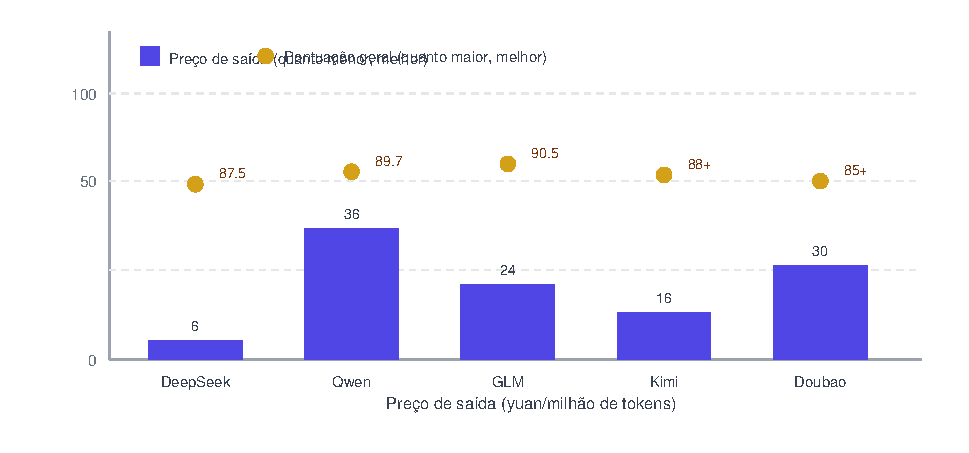
\includegraphics[width=0.92\linewidth]{figures/fig-di-si-shi-er-zhang-1}
\\[2pt]\small Figura 4: comparação de preço e desempenho dos cinco modelos (quanto menor o preço, melhor; quanto maior a pontuação, melhor)
\end{center}

\booksection{Estrutura de decisão para escolher o modelo}

Depois de conhecer as características de cada modelo, como escolher um para o seu projeto? Aqui vai o 'método de decisão das quatro perguntas' — respondendo a quatro questões, você encontra o modelo mais adequado para você.

O projeto será implantado na China ou no exterior?

China escolha um modelo chinês

|

Internacional modelos estrangeiros são uma opção

A tarefa principal é programação ou outra coisa?

Programação Claude ou DeepSeek

|

Outra continuar decidindo

Precisa de contexto extralonga (>500 mil tokens)?

Sim Gemini ou Kimi

|

Não continuar decidindo

O orçamento é um fator?

Sim DeepSeek ou Qwen-turbo

|

Não GPT-5.6 ou Claude

\begin{center}\small\color{gray}Figura 5: método de decisão das quatro perguntas para escolher o grande modelo\end{center}

\begin{tcbinfo}{Dica: estratégia de combinação}
Esse método de decisão não é dogma — muitos cenários pedem a combinação de vários modelos. Uma estratégia comum: DeepSeek ou Qwen para o desenvolvimento do dia a dia (barato e bom com chinês), Claude para o desenho das arquiteturas críticas (raciocínio forte e poucas alucinações) e Gemini para análise multimodal (imagem e vídeo). Troque de modelo conforme a necessidade, em vez de 'usar um só modelo até o fim'.

\end{tcbinfo}

\booksection{Introdução às chamadas de API: conectando-se a grandes modelos do zero}

Muitos tutoriais de programação com IA ensinam apenas a usar a interface de conversa, mas a verdadeira 'programação com IA' — fazer a sua aplicação chamar grandes modelos — exige uma API. A API (Application Programming Interface, interface de programação de aplicativos) é um protocolo de comunicação entre programas. Por meio da API, seu código pode invocar a capacidade de um grande modelo como se chamasse uma função.

\booksubsection{O que é Token}

Antes de entender a API, é preciso compreender o conceito de 'Token'. O Token é a unidade básica de cobrança dos grandes modelos; você pode entendê-lo como a 'unidade de leitura e escrita da IA'. Um Token corresponde, aproximadamente, a 0,75 palavra em inglês (4 caracteres) e a 0,5 a 1 caractere em chinês. Um texto em chinês de 1.000 caracteres consome cerca de 1.500 a 2.000 Tokens.

Token não é número de palavras nem de caracteres. Os grandes modelos usam um tokenizador (Tokenizer) próprio para fatiar o texto em Tokens. A mesma palavra pode ter quantidades diferentes de Tokens em modelos diferentes — por exemplo, 'inteligência artificial' pode virar 3 Tokens no GPT e 2 no DeepSeek. A API da maioria dos modelos devolve a quantidade de Tokens realmente consumida, e você pode conferir isso na resposta.

\begin{tcbinfo}{Estimativa rápida de custo em Tokens}
1 milhão de caracteres em chinês equivale a aproximadamente 1,5 milhão de Tokens. Processar 1 milhão de caracteres de entrada + 1 milhão de caracteres de saída com o DeepSeek V4 Flash custa cerca de US\$ 0,42 (aproximadamente 3 yuans); a mesma quantidade com o Claude Fable 5 custa cerca de US\$ 60 (aproximadamente 434 yuans). É por isso que a escolha do modelo impacta diretamente o custo do seu projeto.

\end{tcbinfo}

\booksubsection{Como obter a API Key}

O primeiro passo para usar a API de grandes modelos é obter a API Key — uma chave usada para autenticar você. Cada provedor de modelos tem a sua plataforma de API, e você precisa criar uma conta e gerar a API Key. A seguir, os portais das plataformas de API dos principais modelos e o passo a passo para obter a chave:

\begin{center}
\begin{tabularx}{\linewidth}{|X|X|X|X|}
\hline
\textbf{Modelo} & \textbf{Plataforma de API} & \textbf{Como obter} & \textbf{Cota gratuita} \tabularnewline
\hline
DeepSeek & platform.deepseek.com & Cadastro verificação de identidade criar API Key & Cota de boas-vindas para novos usuários \tabularnewline
Tongyi Qianwen (Qwen) & bailian.aliyun.com (plataforma Bailian) & Login com conta Alibaba Cloud ativar o serviço criar a Key & Avaliação gratuita para novos usuários \tabularnewline
Zhipu GLM & open.bigmodel.cn & Cadastro verificação de identidade criar API Key & Cota de boas-vindas para novos usuários \tabularnewline
Kimi & platform.moonshot.cn & Cadastro verificação de identidade criar API Key & Cota gratuita limitada \tabularnewline
Doubao & volcengine.com (Volcano Engine) & Cadastro ativar o Ark criar API Key & Muitos Tokens grátis no cadastro \tabularnewline
OpenAI GPT & platform.openai.com & Cadastro vincular cartão de crédito criar API Key & Sem cota gratuita (requer pagamento) \tabularnewline
Anthropic Claude & console.anthropic.com & Cadastro vincular cartão criar API Key & Pequena cota para novos usuários \tabularnewline
\hline
\end{tabularx}
\end{center}

\begin{center}\small\color{gray}Plataformas de API dos principais modelos e como obter a Key (agosto de 2026)\end{center}

\textbf{Dica de segurança: API Key = senha da carteira}\par

A API Key equivale à senha da sua carteira — qualquer pessoa que conseguir a Key pode usar a sua cota para chamar os modelos. Portanto: nunca escreva a API Key no código (gerencie-a com variáveis de ambiente); nunca envie ao Git um código que contenha a Key em repositórios públicos; nunca compartilhe em redes sociais capturas de tela com a Key à mostra. Se a Key vazar, exclua-a imediatamente na plataforma e crie outra.

\booksubsection{Sua primeira chamada de API}

Com a API Key em mãos, você pode chamar a API de grandes modelos em qualquer linguagem de programação. Abaixo, em Python, a chamada mais simples possível — enviar uma mensagem ao DeepSeek e receber a resposta.

\begin{lstlisting}[language=Python]
# Instale o SDK: pip install openai
# O DeepSeek é compatível com o formato do SDK da OpenAI — use direto
from openai import OpenAI
import os

# 1. Crie o client (a API key é lida de uma variável de ambiente)
client = OpenAI(
    api_key=os.environ.get("DEEPSEEK_API_KEY"),
    base_url="https://api.deepseek.com"
)

# 2. Enviar a requisição
response = client.chat.completions.create(
    model="deepseek-chat",  # escolher o modelo
    messages=[
        {"role": "system", "content": "Você é um assistente de programação em Python."},
        {"role": "user", "content": "Escreva uma função de quicksort."}
    ]
)

# 3. Obter a resposta
print(response.choices[0].message.content)

# 4. Conferir o consumo de tokens
print(f"Tokens de entrada: {response.usage.prompt_tokens}")
print(f"Tokens de saída: {response.usage.completion_tokens}")
print(f"Tokens totais: {response.usage.total_tokens}")
\end{lstlisting}

A lógica central desse código é: criar o cliente (com a API Key e o endereço do modelo) montar a lista de mensagens (system define o papel, user é a entrada do usuário) enviar a requisição receber a resposta. Esse padrão funciona com praticamente todos os modelos compatíveis com o formato OpenAI — basta trocar api\_key e base\_url para mudar de modelo. É por isso que muitos modelos nacionais optam por ser compatíveis com o formato do SDK da OpenAI: o desenvolvedor muda duas linhas de código para trocar de modelo, com custo de migração mínimo.

Abaixo estão as diferenças no código para trocar para outros modelos — repare que bastam duas linhas:

\begin{lstlisting}[language=Python]
# DeepSeek
client = OpenAI(
    api_key=os.environ.get("DEEPSEEK_API_KEY"),
    base_url="https://api.deepseek.com"
)
# model="deepseek-chat"

# Qwen (Tongyi Qianwen, plataforma Bailian)
client = OpenAI(
    api_key=os.environ.get("DASHSCOPE_API_KEY"),
    base_url="https://dashscope.aliyuncs.com/compatible-mode/v1"
)
# model="qwen-plus"

# Zhipu GLM
client = OpenAI(
    api_key=os.environ.get("GLM_API_KEY"),
    base_url="https://open.bigmodel.cn/api/paas/v4"
)
# model="glm-4"

# OpenAI GPT
client = OpenAI(
    api_key=os.environ.get("OPENAI_API_KEY"),
    # o base_url padrão serve
)
# model="gpt-5.6-terra"
\end{lstlisting}

\booksubsection{Processamento de respostas em streaming}

Em aplicações reais, você geralmente não quer esperar a IA terminar de escrever tudo para exibir de uma vez — isso faz o usuário esperar demais. As respostas em streaming (Streaming) permitem exibir o texto palavra por palavra enquanto a IA gera, o que melhora muito a experiência do usuário. É como uma máquina de escrever: as palavras vão aparecendo uma a uma, e a sensação para o usuário é completamente diferente.

\begin{lstlisting}[language=Python]
# Streaming: saída caractere por caractere
stream = client.chat.completions.create(
    model="deepseek-chat",
    messages=[
        {"role": "user", "content": "Escreva um tutorial sobre bubble sort em Python"}
    ],
    stream=True  # ativar o streaming
)

# Recebe bloco por bloco e imprime
for chunk in stream:
    if chunk.choices[0].delta.content is not None:
        print(chunk.choices[0].delta.content, end="", flush=True)
# A saída aparece caractere por caractere, como uma máquina de escrever
\end{lstlisting}

\booksection{Guia de compra de Token Plan}

A maioria dos provedores de modelos tem duas formas de cobrança: pagamento por uso (Pay-as-you-go) e assinatura de pacotes (Token Plan / Subscription). Entender a diferença entre elas pode reduzir bastante o seu custo de uso.

\booksubsection{Pagamento por uso vs. assinatura}

\begin{center}
\begin{tabularx}{\linewidth}{|X|X|X|}
\hline
\textbf{Dimensão} & \textbf{Pagamento por uso (Pay-as-you-go)} & \textbf{Assinatura de pacote (Subscription)} \tabularnewline
\hline
Forma de cobrança & Paga pelos Tokens que usar & Pré-paga um valor fixo e recebe uma cota \tabularnewline
Cenários ideais & Consumo instável, chamadas ocasionais & Consumo estável, chamadas frequentes \tabularnewline
Vantagem de preço & Preço padrão & 20\% a 50\% mais barato que o pagamento por uso \tabularnewline
Flexibilidade & Disponível a qualquer momento, sem compromisso & Exige pré-pagamento; a cota pode expirar e se perder \tabularnewline
Tratamento do excedente & Cobrança automática por uso & Depois de estourar a cota, passa a cobrar por uso \tabularnewline
Plataformas representativas & Plataformas de API oficiais de cada modelo & OpenAI Plus/Pro, Claude Pro, Cursor Pro \tabularnewline
\hline
\end{tabularx}
\end{center}

\begin{center}\small\color{gray}Comparação entre as duas formas de cobrança\end{center}

Para iniciantes, a recomendação é começar com pagamento por uso — sem pré-pagamento, você paga pelo que usar. Quando o seu consumo mensal estabilizar em um patamar (por exemplo, mais de 50 yuans por mês), considere migrar para a assinatura de pacote para conseguir um preço unitário menor.

\booksubsection{Visão geral dos principais pacotes de assinatura}

\begin{center}
\begin{tabularx}{\linewidth}{|X|X|X|X|}
\hline
\textbf{Pacote} & \textbf{Mensalidade} & \textbf{O que inclui} & \textbf{Para quem é} \tabularnewline
\hline
ChatGPT Free & Grátis & Conversas de texto ilimitadas com o GPT-5.6 Luna & Experiência para iniciantes \tabularnewline
ChatGPT Plus & US\$ 20/mês & GPT-5.6 Sol, geração de imagens, análise de dados e acesso a plugins & Usuários moderados \tabularnewline
ChatGPT Pro & US\$ 200/mês & Uso ilimitado de todos os modelos e acesso prioritário a novos recursos & Usuários profissionais intensivos \tabularnewline
Claude Free & Grátis & Número limitado de conversas com o Claude & Experiência para iniciantes \tabularnewline
Claude Pro & US\$ 20/mês & Uso ilimitado do Claude e acesso prioritário a novos modelos & Desenvolvedores \tabularnewline
Cursor Free & Grátis & Número limitado de completions de IA e de conversas & Experiência para quem está começando \tabularnewline
Cursor Pro & US\$ 20/mês & Completions de IA ilimitadas, 500 solicitações premium por mês & Desenvolvedores do dia a dia \tabularnewline
Cursor Business & US\$ 40/mês por pessoa & Colaboração em equipe, painel de administração e modo de privacidade & Equipes \tabularnewline
\hline
\end{tabularx}
\end{center}

\begin{center}\small\color{gray}Pacotes de assinatura das principais ferramentas de IA (agosto de 2026)\end{center}

Os esquemas de assinatura dos modelos nacionais são um pouco diferentes. A DeepSeek cobra principalmente por uso e não tem pacote de assinatura mensal — depois de recarregar, você é cobrado pelo consumo real. O Tongyi Qianwen (Qwen) oferece pacotes pré-pagos na plataforma Bailian (comprando uma certa quantidade de cota de tokens com preço com desconto). O Doubao também tem um esquema pré-pago parecido no Volcano Engine. Para os desenvolvedores na China, a combinação mais econômica costuma ser: DeepSeek por uso (desenvolvimento diário) + cota gratuita do Doubao (testes e experimentos).

\booksubsection{Plataformas agregadoras de API}

Se você precisa usar vários modelos ao mesmo tempo, uma plataforma agregadora de API é uma opção sem dor de cabeça. A plataforma agregadora fornece uma única API Key com a qual você chama dezenas de modelos do mundo todo, sem precisar se registrar separadamente em cada plataforma.

\begin{center}
\begin{tabularx}{\linewidth}{|X|X|X|X|}
\hline
\textbf{Plataforma} & \textbf{Características} & \textbf{Vantagem de preço} & \textbf{Cenários ideais} \tabularnewline
\hline
OpenRouter (openrouter.ai) & Agregador internacional: com uma única Key, chama modelos do mundo todo & Preços transparentes, com comparação em tempo real & Quem precisa alternar com flexibilidade entre vários modelos internacionais \tabularnewline
SiliconFlow (siliconflow.cn) & Agregador chinês: oferece APIs de vários modelos nacionais & 20\% a 30\% mais barato que o oficial & Desenvolvedores na China que comparam preços entre modelos \tabularnewline
Azure OpenAI (via Microsoft) & API da OpenAI intermediada pelo Azure da Microsoft & Batch API com 50\% de desconto & Chamadas OpenAI corporativas, tarefas assíncronas em grande volume \tabularnewline
Baidu Qianfan (qianfan.baidubce.com) & Plataforma de nuvem de IA da Baidu, com modelos como o Wenxin (ERNIE) & Cota de boas-vindas para novos usuários & Usuários do ecossistema Baidu \tabularnewline
\hline
\end{tabularx}
\end{center}

\begin{center}\small\color{gray}Principais plataformas agregadoras de API (agosto de 2026)\end{center}

\textbf{Cuidado com a cilada: não compre 'Keys compartilhadas'}\par

Não compre as tais 'API Keys compartilhadas' em plataformas como Taobao ou Xianyu — essas Keys costumam ter origem duvidosa, podem ser banidas a qualquer momento e ainda oferecem risco de vazamento de dados. Obtenha sempre a API Key por plataformas oficiais ou agregadores idôneos.

\booksubsection{Estratégias de otimização de custos}

Escolher o modelo certo é só o primeiro passo; saber 'usar de jeito econômico' importa tanto quanto. A seguir, algumas estratégias de otimização de custo comprovadas na prática:

\begin{enumerate}
  \item Aproveite bem o cache hit. Muitos modelos oferecem o recurso de 'cache' — quando a sua requisição inclui conteúdo já processado antes (como o prompt de sistema), essa parte é cobrada a um preço baixíssimo. No DeepSeek, o preço de cache hit é apenas 1/60 do preço normal. Colocar o prompt de sistema fixo no começo da lista de mensagens maximiza o cache hit.
  \item Roteamento em níveis — use modelos baratos nas tarefas simples e modelos caros nas tarefas complexas. Por exemplo, use o DeepSeek V4 Flash para classificação de texto (saída de 2 yuans/1M de tokens) e o Claude para o desenho de arquitetura (saída de 181 yuans/1M de tokens). Em um projeto, 80\% das chamadas podem usar o modelo barato.
  \item Limite o tamanho da saída. A API cobra pelos Tokens de saída; quanto mais longa a saída, mais caro. Em cenários que não pedem discursos longos, defina o parâmetro max\_tokens para limitar o tamanho da saída e evitar que a IA 'fale demais'.
  \item Use a Batch API nas tarefas que não são em tempo real. Se você tem muitas tarefas que não precisam de resposta imediata (como anotação de dados em lote e resumos de documentos), a Batch API dá 50\% de desconto. A OpenAI e a Azure oferecem esse recurso.
  \item Monitore o consumo de Tokens. A maioria das plataformas de API oferece painéis de estatísticas de uso. Confira periodicamente a distribuição do consumo, descubra as chamadas que mais gastam Tokens e otimize pontualmente. Um pequeno ajuste no prompt (por exemplo, trocar 'explique em detalhes' por 'explique em 3 frases') pode economizar 50\% dos Tokens.
\end{enumerate}

\begin{center}
\begin{tabularx}{\linewidth}{|X|X|X|X|}
\hline
\textbf{Estratégia} & \textbf{Economia} & \textbf{Dificuldade} & \textbf{Observação} \tabularnewline
\hline
Cache hit & Até 98\% & Baixo & Coloque o conteúdo fixo no começo das mensagens \tabularnewline
Roteamento em níveis & 50\%-80\% & Médio & Use modelos baratos nas tarefas simples \tabularnewline
Limitar o tamanho da saída & 30\%-60\% & Baixo & Definir o parâmetro max\_tokens \tabularnewline
Batch API & 50\% & Baixo & Use processamento em lote nas tarefas não imediatas \tabularnewline
Otimização de prompt & 20\%-50\% & Médio & Prompt enxuto, com menos redundância \tabularnewline
\hline
\end{tabularx}
\end{center}

\begin{center}\small\color{gray}Estratégias de otimização de custo e seus efeitos (agosto de 2026)\end{center}

\booksection{Prática: conectando a API de grandes modelos em um projeto}

Vamos encerrar o capítulo com uma prática completa — criar um 'Gerador de Resumos com IA': o usuário insere um texto longo e a aplicação chama a API de um grande modelo para gerar o resumo. Essa prática mostra o fluxo completo de uma chamada de API: configuração do ambiente, chamada, tratamento de erros e controle de custos.

\begin{lstlisting}[language=Python]
# ai_summarizer.py - Resumidor de IA
import os
from openai import OpenAI

# 1. Configurar (a API key é lida de uma variável de ambiente — nunca hardcode)
client = OpenAI(
    api_key=os.environ.get("DEEPSEEK_API_KEY"),
    base_url="https://api.deepseek.com"
)

def summarize(text: str, max_length: int = 200) -> dict:
    """Gera o resumo de um texto

    Args:
        text: o texto original a resumir
        max_length: tamanho máximo do resumo (em tokens)

    Returns:
        dict: resumo mais informações de consumo de tokens
    """
    try:
        response = client.chat.completions.create(
            model="deepseek-chat",
            messages=[
                {
                    "role": "system",
                    "content": "Você é um gerador de resumos."
                               "Resuma de forma concisa o texto fornecido pelo usuário."
                               "O resumo não passe de 3 frases."
                },
                {
                    "role": "user",
                    "content": f"Resuma o seguinte texto:\n\n{text}"
                }
            ],
            max_tokens=max_length,  # limita o tamanho da saída
            temperature=0.3  # temperatura baixa = mais estável
        )

        return {
            "success": True,
            "summary": response.choices[0].message.content,
            "input_tokens": response.usage.prompt_tokens,
            "output_tokens": response.usage.completion_tokens,
            "total_tokens": response.usage.total_tokens
        }

    except Exception as e:
        return {
            "success": False,
            "error": str(e)
        }

# 2. Exemplo de uso
if __name__ == "__main__":
    long_text = """
    (cole aqui um texto longo...)
    """

    result = summarize(long_text)

    if result["success"]:
        print(f"Resumo: {result['summary']}")
        print(f"Tokens usados: {result['total_tokens']}")
        # estimativa de custo: DeepSeek V4 Flash
        cost = result['total_tokens'] * 0.000004  # $\approx$0,4 fen por 1.000 tokens
        print(f"Custo estimado: {cost:.4f} yuan")
    else:
        print(f"Erro: {result['error']}")
\end{lstlisting}

Esse código incorpora várias boas práticas de chamada de API: a API Key é lida de variáveis de ambiente, nunca escrita direto no código; as funções têm documentação e type hints claros; o max\_tokens limita o tamanho da saída; o temperature está em um valor baixo (0,3) para gerar uma saída mais estável; há tratamento completo de erros; e são devolvidas as informações de consumo de Tokens para rastrear custos. Quando pedir à IA que escreva esse código, você pode passar esses requisitos — ela é totalmente capaz de implementá-los.

A lição final do capítulo: modelos são a "munição", a metodologia é a "tática". A munição certa facilita a batalha, mas sem uma boa tática nem a melhor munição vence a guerra. Agora que você conhece as características de cada modelo e como usar as APIs, tem um "arsenal" completo — mas como travar essa batalha depende dos métodos de pensamento dos capítulos anteriores.

\begin{tcbpractice}{Mãos à obra: coloque sua primeira chamada de API para funcionar}
Cadastre-se em uma plataforma de modelos nacional (recomendamos DeepSeek ou Zhipu — as duas dão cota para novos usuários), crie a API Key, coloque-a nas variáveis de ambiente do sistema (não no código!) e execute o código de 'sua primeira chamada de API' acima. No momento em que vir a resposta da IA impressa na tela, você terá cruzado a linha que separa 'usar IA' de 'construir aplicações com IA'.

\end{tcbpractice}

\begin{tcbsummary}{Resumo do capítulo}
\begin{itemize}
  \item Os três fortes internacionais: GPT-5.6 (equilibrado e versátil), Claude (o topo da programação + taxa de alucinação de apenas 1\%) e Gemini (o rei do multimodal + contexto de 2 milhões)
  \item Os cinco fortes nacionais: DeepSeek V4 (o rei do custo-benefício; fique de olho no aviso de reajuste), Qwen3.7 (corporativo), GLM-5.1 (nº 1 da China em SWE), Kimi K3 (textos ultralongos) e Doubao (comece grátis)
  \item Método das quatro perguntas: onde será implantado? É programação ou outra coisa? Precisa de contexto ultralongo? O orçamento é sensível?
  \item Token é a unidade de cobrança: 1 caractere em chinês equivale a cerca de 1,5 a 2 Tokens; 1 milhão de caracteres equivale a cerca de 1,5 milhão de Tokens
  \item API Key = senha da carteira: gerencie com variáveis de ambiente, nunca escreva no código e nunca envie ao Git
  \item Os modelos nacionais são, em geral, compatíveis com o SDK da OpenAI: para trocar de modelo, basta alterar duas linhas — api\_key e base\_url
  \item Cinco truques para economizar: cache hit, roteamento em níveis, limite de saída, Batch API e monitoramento do consumo
\end{itemize}

\end{tcbsummary}
